\documentclass[12pt,a4paper]{article}
\usepackage[utf8]{inputenc}
\usepackage[ngerman]{babel}
\usepackage{graphicx}
\usepackage{fancyhdr}
\usepackage{titlesec}
\usepackage{parskip}
\usepackage{xcolor}
\usepackage{csquotes}
\usepackage{lastpage}
\usepackage[margin=2.5cm,headheight=16pt]{geometry}
\usepackage{verbatim}

% header/footer
\pagestyle{fancy}
\fancyhf{}
\lhead{Matthes Elstermann, Lukas Gnad}
\rhead{Windows certificate import}
\cfoot{Seite \thepage~von \pageref{LastPage}}

% section
\titleformat{\section}{\normalfont\bfseries\large}{}{0pt}{}

\begin{document}

% title
\begin{center}
  \LARGE{\textbf{Certificate import for Windows to\\install ALPS Visio Plugin}}\\
  \medskip
  \normalsize{Matthes Elstermann, Lukas Gnad}
\end{center}

\vspace{1.5em}
\hrule
\vspace{1.5em}

\section*{Read before installation}

The ALPS-Visio plugin is a Windows plugin which can only be installed if the plugins certificate is trusted by the Windows System. The certificate which was used to sign the ALPS-plugin is a testing certificate, so common Windows systems will not accept it as certificate of a trusted authority. To achieve this, the certificate can be loaded into the \enquote{trusted root certificates} folder manually. However, this might be a \textbf{potential security risk} for Windows system, and it is \textbf{highly recommended} to remove the certificate after a successful installation.

\section*{Installing the certificate}

The install the certificate used for signing the plugin, move to the plugin directory and right-click onto the \enquote{setup.exe}. Choose \enquote{Properties}.

\begin{center}
  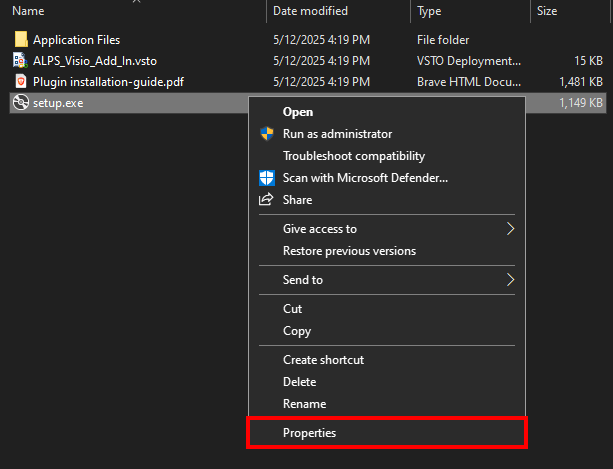
\includegraphics[width=0.8\linewidth]{images/properties.png}
\end{center}

In the new window, choose the tab \enquote{Digital signatures}.

Under \enquote{Signature list}, choose the certificate and click on \enquote{Details}.

\begin{center}
  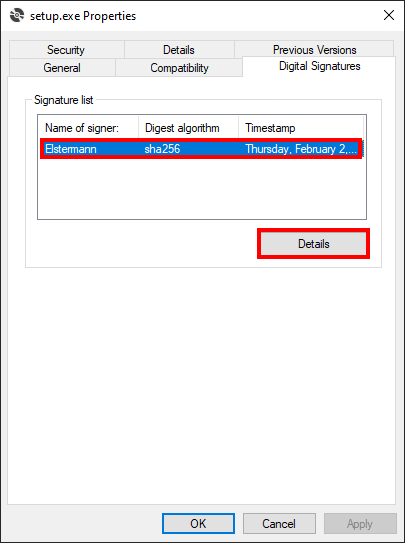
\includegraphics[width=0.8\linewidth]{images/details.png}
\end{center}

Under \enquote{Signer information}, choose \enquote{View Certificate}:

\begin{center}
  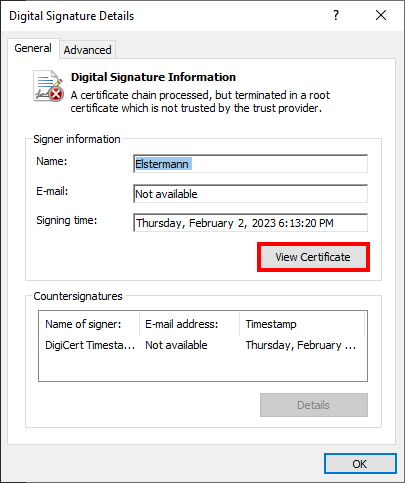
\includegraphics[width=0.8\linewidth]{images/view_certificate.png}
\end{center}

And in the next window, \enquote{Install Certificate...}:

\begin{center}
  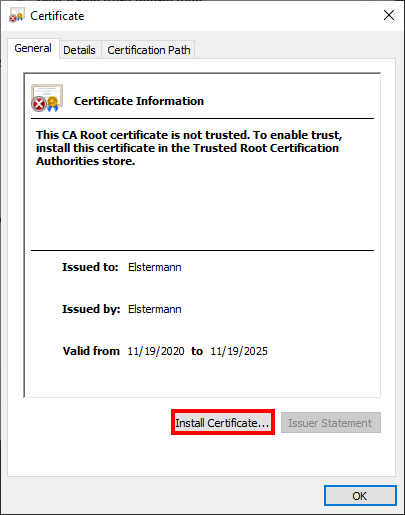
\includegraphics[width=0.8\linewidth]{images/install_certificate.png}
\end{center}

The Certificate Import Wizard will pop up.

\textbf{First page:}

The certificate should be installed for the current user only, as it should not affect the installing behavior of other users on the system.

Choose \enquote{current user} and go ahead.

\begin{center}
  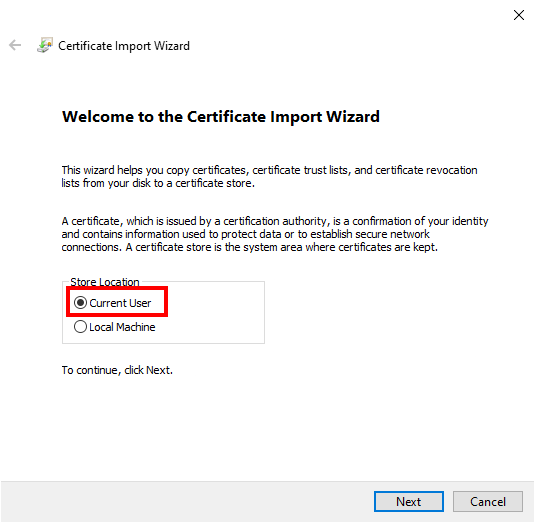
\includegraphics[width=0.8\linewidth]{images/installer_1.png}
\end{center}

\textbf{Second page:}

As stated before, the used certificate is only a test certificate. If it is up to Windows to decide where to store the imported certificate, windows will choose a folder where the certificate is stored, but used as trusted certificate when it comes to software installation.

To be able to install the plugin correctly, \enquote{Place all certificates in the following store:} must be selected
and the \enquote{Trusted Root Certification Authorities} store must be chosen.

\begin{center}
  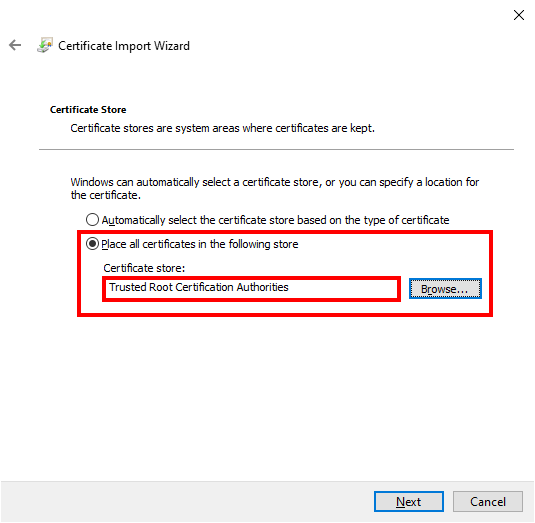
\includegraphics[width=0.8\linewidth]{images/installer_2.png}
\end{center}

\textbf{Third page:}

Windows will display a warning that it cannot validate this certificate, and that you install at your
own risk.

Click yes and finish the installation.

\begin{center}
  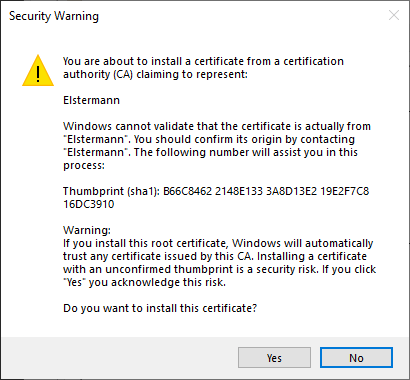
\includegraphics[width=0.8\linewidth]{images/installer_3.png}
\end{center}

\section*{Allow windows to access the Installer}

It can happen that the installation fails with the error \enquote{The deployment and application do not have matching security zones.}

\begin{center}
  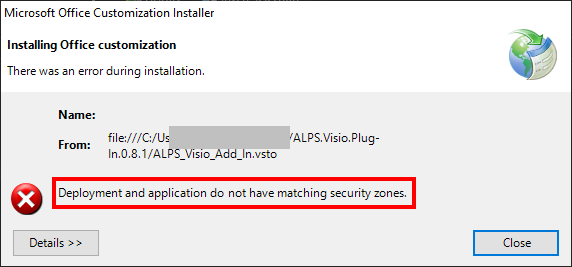
\includegraphics[width=0.8\linewidth]{images/error.png}
\end{center}

If you encounter this error, you can manually unblock the files.

For \textbf{every file} (including those in subfolders):
\begin{itemize}
  \item Right-click the file and choose \enquote{Properties}.
  \item If you see a message at the bottom that says \enquote{This file came from another computer and might be blocked.}, check \enquote{Unblock}, then click \enquote{Apply} and \enquote{OK}.
\end{itemize}

\begin{center}
  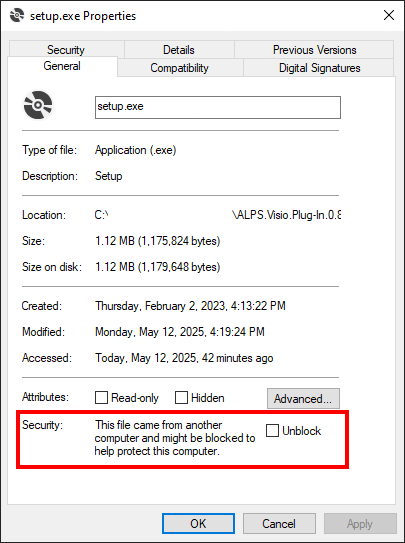
\includegraphics[width=0.8\linewidth]{images/unblock.png}
\end{center}

\textbf{Automated Solution:}

Instead of unblocking all files manually, you can also use this script to unblock all files automatically:

\begin{verbatim}
FOR %a in (*.*) do (echo.>%a:Zone.Identifier)
FOR %a in ("Application Files\ALPS_Visio_Add_In_1_0_0_241\*.*")
        do (echo.>%a:Zone.Identifier)
FOR %a in ("Application Files\ALPS_Visio_Add_In_1_0_0_242\*.*")
        do (echo.>%a:Zone.Identifier)
\end{verbatim}

To run it, open a terminal in the \enquote{ALPS.Visio.Plug-In.0.8.1} Folder and execute the lines of code one at a time.

\begin{center}
  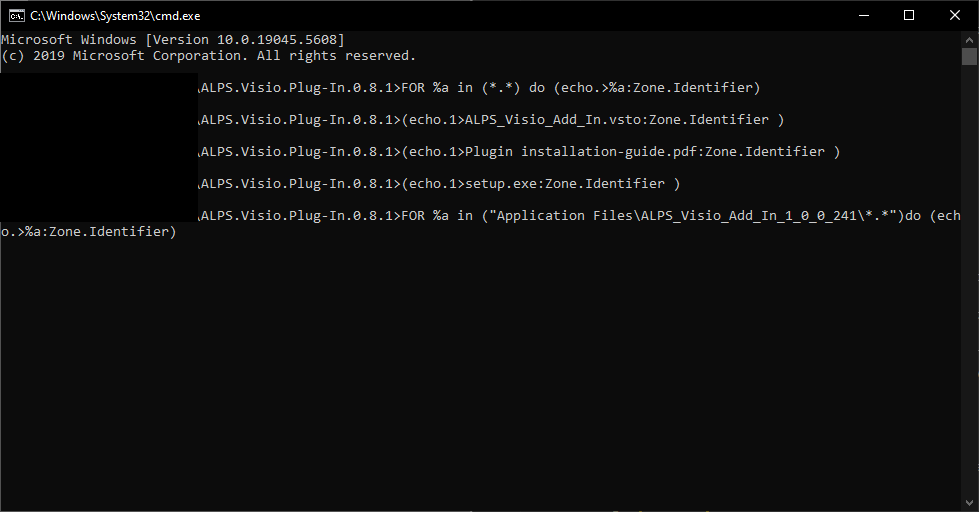
\includegraphics[width=0.8\linewidth]{images/console_3.png}
\end{center}

Close all the windows and install the plugin.

It is recommended to delete the certificate afterwards immediately (See next section).

\newpage

\section*{Removing the installed certificate}

There are two possible locations for the certificate, depending on what was chosen when importing the certificate:
\begin{enumerate}
  \item The certificate has been installed for the current user only:
  
  Open the windows search bar and type \enquote{Manage user certificates}.
  \item The certificate has been installed for the whole system:
  
  Open the windows search bar and type \enquote{Manage computer certificates}.
\end{enumerate}

\begin{center}
  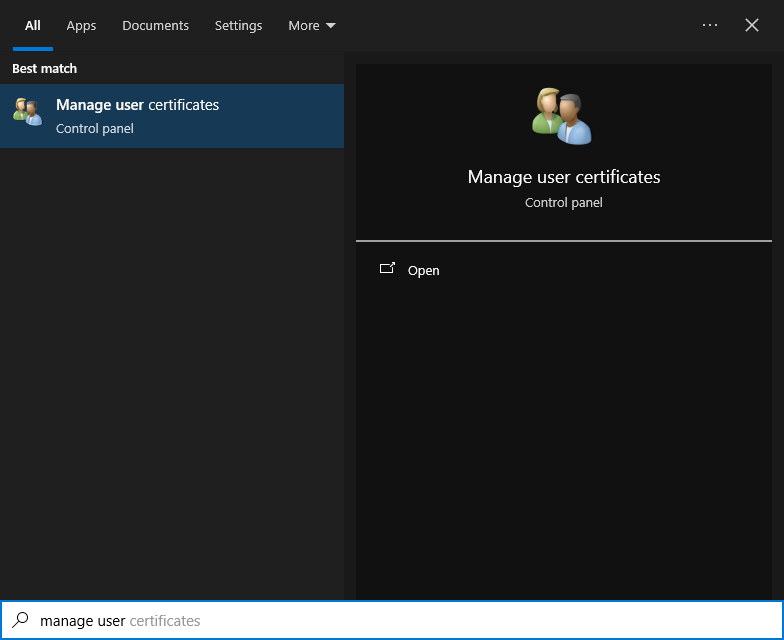
\includegraphics[width=0.8\linewidth]{images/manage_user_certificates.png}
\end{center}

In the \texttt{certmgr}-window, chose \enquote{Trusted Root Certification Authorities}, then \enquote{Certificates} in the overview on the left. Here the installed certificate can be found and deleted.

\begin{center}
  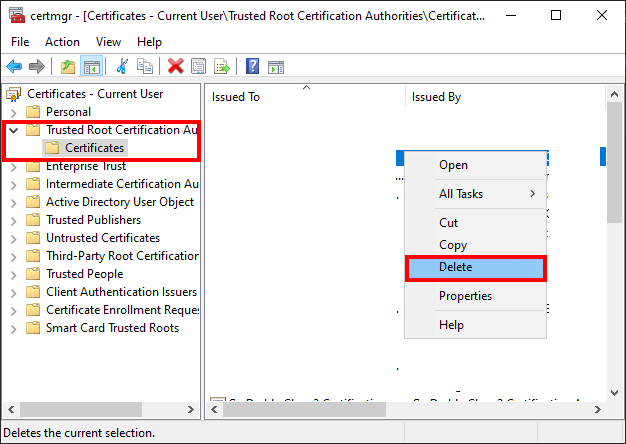
\includegraphics[width=0.8\linewidth]{images/delete_certificate.png}
\end{center}

\end{document}
